\section{実験}
\subsection{共通設定}
評価にはCOCO 2017 Validation（5000枚）を用いた．
閾値の選択と結果の報告に同じ画像を用いないよう，seed 42でサンプリングした500枚（以下，dev500）を検証用とし，残りの4500枚を2等分した後半からサンプリングした500枚（以下，test500，GTインスタンス3748件）をテスト用とした．
細かい粒度の評価には，WordNetのSynsetが各カテゴリに付与されたLVIS v1\cite{ref_LVIS}のValidationのアノテーションを用いた．
LVISのアノテーションはCOCO 2017の画像に付与されており，5000枚のうち4809枚に存在する．
dev500と前述の4500枚の前半のうちLVISのアノテーションが存在する2604枚を検証用（以下，lvis\_dev），後半の2148枚をテスト用（以下，lvis\_test）とした．
VLMにはSigLIP-ViT-B/16（WebLIで学習）を，検出器にはDETR（ResNet-50）とYOLO11xを用いた．
DETRの閾値$ \theta $とYOLO11xの閾値は，評価インスタンス数が近くなる組として，$ \theta = 0.5 $とYOLO11xの0.25を主に示す．
GPUにはNVIDIA GeForce RTX 4070 Tiを用い，いずれの手法も追加の学習は行わない．

検出ボックスとCOCOのGTは，IoUが0.5以上の組をハンガリアン法で1対1に対応付けた．
対応したインスタンスについて，深さ0の語がGTのカテゴリと一致する割合をTop-1正解率，深さ0が正解のインスタンス数をGTインスタンスの総数で割った値を正命名率$ r $とした．
また，深さ0が正解であり，かつ下位語を持つため粒度を変更できたインスタンス数を$ N_h $とした．

深さ1以降の評価には，COCOのGTに対応した検出ボックスについて，IoUが0.5以上で，そのSynsetがGTカテゴリのSynsetの真の下位語であるLVISのアノテーションを細かい粒度の正解とした．
例えば，COCOのbirdに対するpigeonである．
インスタンス$ k $について，出力した各段階のSynsetの集合を$ {\mathbb P}_k $，GTカテゴリのSynsetからLVISのSynsetまでの経路上のSynsetの集合を$ {\mathbb G}_k $とし，階層的適合率と階層的再現率\cite{ref_hF}を

\begin{equation}
    hP = \frac{\sum_k |{\mathbb P}_k \cap {\mathbb G}_k|}{\sum_k |{\mathbb P}_k|}, \quad
    hR = \frac{\sum_k |{\mathbb P}_k \cap {\mathbb G}_k|}{\sum_k |{\mathbb G}_k|}
    \label{eq_hierarchical_pr}
\end{equation}

\noindent
とし，その調和平均を$ hF $とした．
LVISのSynsetより細かいSynsetは正誤を判定できないため$ {\mathbb P}_k $から除き，棄却したインスタンスでは$ {\mathbb P}_k = \emptyset $とした．
(\ref{eq_cumulative})の$ \tau $は，lvis\_devで$ hF $が最大となる値を$ 0 $から$ 0.9 $の16通りから選んだ．

\subsection{COCOにおける3つの構成の比較}
表\ref{tab_coco}に，test500における深さ0の結果を示す．

\begin{table}[t]
    \centering
    \caption{test500における深さ0の評価．閾値は提案手法ではDETRの$ \theta $，YOLO11x単体とハイブリッド手法ではYOLO11xの検出スコアの閾値，$ n $は評価インスタンス数，$ N_h $は深さ0が正解で粒度を変更できたインスタンス数である．}
    \label{tab_coco}
    \footnotesize
    \setlength{\tabcolsep}{3pt}
    \begin{tabular}{lccccc}
        \toprule
        手法 & 閾値 & $ n $ & Top-1 & $ r $ & $ N_h $ \\
        \midrule
        YOLO11x単体  & 0.25 & 2572 & 0.969 & 0.665 & 0 \\
        提案手法     & 0.5  & 2736 & 0.527 & 0.385 & 1219 \\
        ハイブリッド & 0.25 & 2572 & 0.969 & 0.665 & 2187 \\
        \midrule
        YOLO11x単体  & 0.7  & 1584 & 0.982 & 0.415 & 0 \\
        提案手法     & 0.97 & 1669 & 0.609 & 0.271 & 867 \\
        ハイブリッド & 0.7  & 1584 & 0.982 & 0.415 & 1360 \\
        \bottomrule
    \end{tabular}
\end{table}

表\ref{tab_coco}から，COCOの80クラスの範囲では，YOLO11xのTop-1正解率0.969に対し，DETRとSigLIPによる提案手法は0.527であった．
提案手法の誤りの多くは，COCOで学習されていないSigLIPのゼロショット分類によるものであり，検出数$ n $は同程度である．
ハイブリッド手法は深さ0の精度をYOLO11xと同じに保ったまま，粒度を変更できたインスタンス$ N_h $を，提案手法の1.79倍（閾値0.25と$ \theta = 0.5 $）および1.57倍（閾値0.7と$ \theta = 0.97 $）に増やした．
YOLO11x単体は深さ0の語のみを出力するため，$ N_h = 0 $である．

\subsection{LVISによる細かい粒度の評価}
表\ref{tab_lvis}と図\ref{fig_lvis_stopping}に，lvis\_testにおける深さ1以降の結果を示す．
評価インスタンス数は，提案手法で489件，YOLO11x単体とハイブリッド手法で481件である．
図\ref{fig_lvis_stopping}の横軸は$ hR $，縦軸は$ hP $であり，曲線は$ \tau $を変化させた停止規則，四角は深さの上限（0〜3）で止める規則，星印はlvis\_devで選んだ$ \tau $である．

\begin{table}[t]
    \centering
    \caption{lvis\_testにおける深さ1以降の評価．深さ1は深さ0が正解のインスタンスにおける深さ1の正解率，到達はLVISのSynsetまで細分化できた割合（停止なし）である．$ hF $の停止なしは下位語の集合が空になるまで出力した場合，$ \tau $はlvis\_devで選んだ$ \tau $による停止規則である．}
    \label{tab_lvis}
    \scriptsize
    \setlength{\tabcolsep}{1.6pt}
    \begin{tabular}{lccccccc}
        \toprule
        & & & & \multicolumn{2}{c}{停止なし} & \multicolumn{2}{c}{$ \tau $による停止} \\
        \cmidrule(lr){5-6} \cmidrule(lr){7-8}
        手法 & 確信度 & 深さ1 & 到達 & $ hP $ & $ hF $ & $ hP $ & $ hF $ \\
        \midrule
        YOLO11x単体  & --         & --    & 0.000 & 0.971 & 0.604 & 0.971 & 0.604 \\
        提案手法     & シグモイド & 0.462 & 0.276 & 0.434 & 0.433 & 0.486 & 0.450 \\
        提案手法     & ソフトマックス & 0.462 & 0.276 & 0.434 & 0.433 & 0.715 & 0.480 \\
        ハイブリッド & シグモイド & 0.405 & 0.389 & 0.602 & 0.619 & 0.757 & 0.659 \\
        ハイブリッド & ソフトマックス & 0.405 & 0.389 & 0.602 & 0.619 & 0.720 & 0.648 \\
        \bottomrule
    \end{tabular}
\end{table}

\begin{figure}[t]
    \centering
    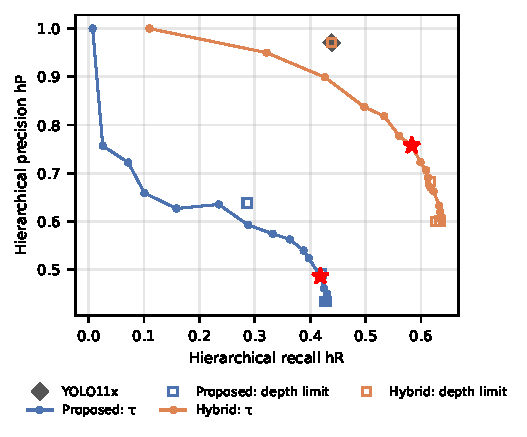
\includegraphics[width=0.9\columnwidth]{figures/fig_lvis_stopping.pdf}
    \caption{lvis\_testにおける階層的再現率$ hR $（横軸）と階層的適合率$ hP $（縦軸）の関係（確信度はシグモイド）．曲線は累積確信度による停止規則，四角は深さの上限（0〜3）による停止規則，星印はlvis\_devで選んだ$ \tau $である．}
    \label{fig_lvis_stopping}
\end{figure}

表\ref{tab_lvis}から，YOLO11x単体は深さ0のみを出力するため$ hP = 0.971 $と高いが，細かい粒度を出力しないため$ hR $は0.438にとどまった．
ハイブリッド手法は，下位語の集合が空になるまで出力すると$ hP $が0.602に下がるが，LVISのSynsetまで細分化できた割合は38.9\%であった．
シグモイドの確信度による停止規則では，$ \tau = 0.05 $で$ hP = 0.757 $，$ hR = 0.583 $となり，$ hF $は0.659とYOLO11x単体の0.604を上回った．
一方，深さ0が正しい場合でも深さ1の推定が正しいのは提案手法で46.2\%，ハイブリッド手法で40.5\%であり，最初の細分化の段階で半数以上を誤った．

確信度の正規化関数の影響を調べるため，深さ0の正誤を最も深い段階の確信度で区別するArea Under the ROC Curve（AUROC）をtest500で求めた．
ハイブリッド手法では，シグモイドで0.617，ソフトマックスで0.480であり，誤った語の下位語のみを候補とする段階でも，シグモイドは画像と語の対応が弱いことを低い確信度として表した．
一方，深さ0が正しい場合の深さ1の正誤を深さ1の確信度で区別するAUROCは，ハイブリッド手法でシグモイドが0.644，ソフトマックスが0.780であり，兄弟の語の間の比較にはソフトマックスが適していた．
提案手法では，シグモイドの深さ0の確信度が小さく，$ \tau $を大きくすると多くのインスタンスが棄却されるため，$ hF $はソフトマックスの0.480に対し0.450であった．

\subsection{COCO外の物体の検出}
YOLO11xやDETRはCOCOで学習されているため，COCO外の物体を背景として扱い，検出しない場合がある．
そこで，lvis\_testの2148枚において，COCOの物体（15842件）と，COCO外の物体（12655件）の検出の再現率を比較した．
COCO外の物体は，LVISのアノテーションのうち，SynsetがCOCOのカテゴリのSynsetの上位語・下位語でなく，レンマ名もCOCOのカテゴリ名と一致しないものである．
比較した検出器は，YOLO11x（閾値0.01），DETR（閾値0.01），OWLv2\cite{ref_OWLv2}（ViT-B/16）のテキストに依存しない物体らしさのスコア，およびテキスト「object.」を与えたGrounding DINO\cite{ref_GroundingDINO}（tiny）である．
いずれもIoU 0.5のクラス非依存のNMSを行い，スコアの上位$ K $件のボックスにIoUが0.5以上のボックスが含まれるGTの割合を再現率とした．

図\ref{fig_recall}に結果を示す．
横軸は1画像あたりのボックス数（対数），縦軸は再現率であり，黒の記号はYOLO11x（閾値0.25）とDETR（$ \theta = 0.5 $）の出力である．

\begin{figure}[t]
    \centering
    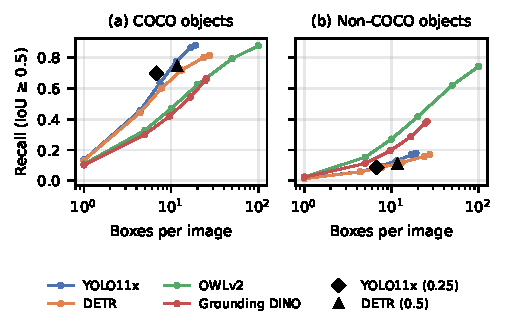
\includegraphics[width=\columnwidth]{figures/fig_recall.pdf}
    \caption{lvis\_testにおける1画像あたりのボックス数（横軸）と再現率（縦軸）の関係．(a)はCOCOの物体，(b)はCOCO外の物体であり，黒の記号はYOLO11x（閾値0.25）とDETR（$ \theta = 0.5 $）の出力である．}
    \label{fig_recall}
\end{figure}

図\ref{fig_recall}(b)から，YOLO11x（閾値0.25）が検出したCOCO外の物体は8.7\%，DETR（$ \theta = 0.5 $）は11.0\%であった．
YOLO11xとDETRは閾値を0.01まで下げても，COCO外の物体の再現率はそれぞれ17.9\%と17.0\%で飽和した．
これに対し，OWLv2の物体らしさのスコアでは，1画像あたり10件で27.1\%，100件で74.3\%であり，Grounding DINO（25.6件で38.5\%）を上回った．
一方，図\ref{fig_recall}(a)から，COCOの物体ではYOLO11xが少ないボックス数で最も高い再現率を示した．
すなわち，COCOの物体にはYOLO11x，COCO外の物体にはOWLv2という役割の分担が有効である．

\subsection{COCO外の物体の命名と粒度の変更}
(\ref{eq_supplement})により，YOLO11x（閾値0.25）のボックスに，各検出器の候補を$ K_{\mathrm{add}} $件加えた構成を評価した．
出力したボックスとGT（COCOの物体とCOCO外の物体）をIoU 0.5以上で1対1に対応付け，COCO外の物体のうち，ボックスと対応した割合（検出），深さ0の語がLVISのSynsetの上位語または自身であった割合（命名），下位語の展開がLVISのSynsetに到達した割合（到達）を求めた．
命名の語彙$ {\mathbb V}_0 $には(\ref{eq_wordnet_vocab})の681語を用い，語彙が既知の場合の参考として，LVISのカテゴリ名（1203語）を語彙とした場合も示す．
提案手法も，DETR（$ \theta = 0.5 $）のボックスを同じ語彙で命名した．
表\ref{tab_open}に$ K_{\mathrm{add}} = 10 $の結果を示す．

\begin{table}[t]
    \vspace{3mm}
    \centering
    \caption{lvis\_testにおけるCOCO外の物体の検出，命名，粒度の変更（$ K_{\mathrm{add}} = 10 $）．COCOはCOCOの物体のうち深さ0が正解の割合，検出・命名・到達はCOCO外の物体12655件に対する割合であり，括弧内はLVISのカテゴリ名を語彙とした場合である．}
    \label{tab_open}
    \scriptsize
    \setlength{\tabcolsep}{1.5pt}
    \begin{tabular}{lcccc}
        \toprule
        構成 & COCO & 検出 & 命名 & 到達 \\
        \midrule
        YOLO11x単体          & 0.649 & 0.046 & 0.000 & 0.000 \\
        ハイブリッド         & 0.649 & 0.046 & 0.000 & 0.000 \\
        提案手法             & 0.231 & 0.070 & 0.006 (0.018) & 0.005 (0.017) \\
        ハイブリッド + YOLO11x & 0.663 & 0.094 & 0.005 (0.011) & 0.005 (0.011) \\
        ハイブリッド + DETR    & 0.660 & 0.087 & 0.004 (0.010) & 0.004 (0.009) \\
        ハイブリッド + OWLv2   & 0.661 & 0.316 & 0.025 (0.084) & 0.023 (0.081) \\
        ハイブリッド + G. DINO & 0.659 & 0.217 & 0.021 (0.057) & 0.019 (0.056) \\
        \bottomrule
    \end{tabular}
\end{table}

表\ref{tab_open}から，YOLO11x単体とハイブリッド手法はCOCO外の物体の4.6\%しか検出せず，検出した物体にもCOCOの語しか与えないため，命名と粒度の変更はいずれも0であった．
OWLv2の候補を加えると，COCO外の物体の検出は31.6\%と6.9倍になり，COCOの物体の正解率も0.649から0.661へわずかに上がった．
すなわち，YOLO11xのボックスと重ならない領域のみを加えることで，COCOの物体に対する精度を損なわずに，検出されなかった物体を粒度の変更の対象にできた．
ただし，検出したCOCO外の物体のうち深さ0を正しく命名できたのは，WordNetの語彙で8.1\%，LVISのカテゴリ名を語彙とした場合でも26.7\%にとどまった．
また，加えたボックスのうちGTと対応したのは21.4\%であり，残りはLVISで注釈されていない物体や物体の部分であった．
$ K_{\mathrm{add}} $を20に増やすと，OWLv2の候補による検出は43.6\%，命名は3.5\%（LVISの語彙で11.1\%）となった．

\begingroup
\color{red}
\subsection{COCO外の物体の命名の改善}
3.7節の棄却と上から下への命名に加え，VLMをSigLIP SO400M（ViT-SO400M-14-SigLIP-384）に変更する構成，クロップのボックスを縦横1.5倍に広げて周辺を含める構成，および深さ1以降のプロンプトに親の語を含める（``a photo of a hound, a type of dog''）構成を評価した．
比較として，(\ref{eq_wordnet_vocab})の語彙から物体の部分を表す語を除き，キャプションに出現する語に限った語彙（COCOの80語を含む435語）を用いる構成も評価した．
YOLO11xのボックスは全構成で共通とし，ハイブリッド手法と同じくシグモイドの累積確信度で$ \tau = 0.05 $まで出力した．

評価には，COCOの物体とCOCO外の物体を合わせた全てのGTと，棄却されなかった全ての出力ボックスを用いた．
出力ボックスとGTをIoU 0.5以上で1対1に対応付け，出力した語とGTのSynsetのそれぞれについて，自身と全ての上位語のうち深さ4以上のSynsetの集合から(\ref{eq_hierarchical_pr})と同様に$ hP $と$ hR $を求めた．
GTと対応しない出力ボックスは$ hP $の分母のみに，対応する出力の無いGTは$ hR $の分母のみに含めた．
したがって，粗い語であっても正しい上位語を出力すれば部分的に正解となり，誤った細かい語は不正解となる．
ただし，LVISの注釈は網羅的でないため，全体の$ hF $が最大となる閾値を選ぶと，加えた候補がほぼ全て棄却される．
そこで，1画像あたりに加える候補の数の上限（予算）$ B $を定め，lvis\_devの1000枚で，予算以下となる閾値の組のうちCOCO外の物体の$ hR $が最大となる組を選び，lvis\_testで評価した．
探索した閾値は，$ K_{\mathrm{add}} \in \{1, 2, 5, 10, 20\} $，$ o \in \{0, 0.1, 0.2, 0.3\} $，$ \gamma \in \{0, 0.003, 0.01, 0.03, 0.1\} $，包含による棄却の有無，$ \tau_s \in \{0, 0.5, 0.7, 0.9\} $および深さ0のみを出力する設定である．

\begin{table}[t]
    \centering
    \caption{lvis\_testにおけるCOCO外の物体の命名の改善．追加は1画像あたりに加えた候補の数，命名はCOCO外の物体12655件のうち深さ0が正しい上位語となった割合，$ hR $はCOCO外の物体の階層的再現率，適合率は加えた候補のうちGTと対応し正しい上位語を出力した割合である．}
    \label{tab_naming}
    \scriptsize
    \setlength{\tabcolsep}{1.4pt}
    \resizebox{\columnwidth}{!}{%
    \begin{tabular}{lcccccccc}
        \toprule
        & \multicolumn{4}{c}{$ B = 2 $} & \multicolumn{4}{c}{$ B = 5 $} \\
        \cmidrule(lr){2-5} \cmidrule(lr){6-9}
        構成 & 追加 & 命名 & $ hR $ & 適合率 & 追加 & 命名 & $ hR $ & 適合率 \\
        \midrule
        上位$ K $件（表\ref{tab_open}）& 2.00 & 0.010 & 0.047 & 0.054 & 5.00 & 0.017 & 0.073 & 0.036 \\
        + 棄却                          & 1.90 & 0.014 & 0.056 & 0.081 & 4.57 & 0.023 & 0.084 & 0.052 \\
        + 上から下への命名               & 1.88 & 0.014 & 0.053 & 0.080 & 4.92 & 0.031 & 0.081 & 0.065 \\
        + SO400M                         & 1.88 & 0.016 & 0.054 & 0.092 & 4.95 & 0.041 & 0.085 & 0.081 \\
        + SO400M，拡大，親の語           & 1.99 & 0.019 & 0.056 & 0.114 & 4.85 & 0.035 & 0.086 & 0.081 \\
        \midrule
        語彙の限定 + SO400M（参考）      & 1.93 & 0.011 & 0.050 & 0.083 & 4.83 & 0.021 & 0.076 & 0.054 \\
        \bottomrule
    \end{tabular}%
    }
\end{table}

\begin{figure}[t]
    \centering
    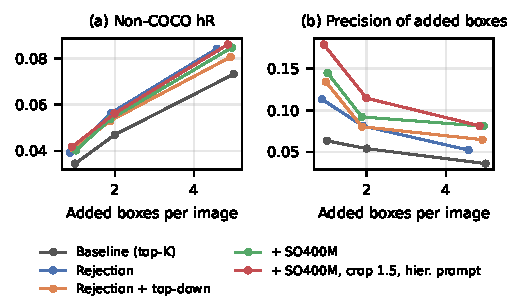
\includegraphics[width=\columnwidth]{figures/fig_budget.pdf}
    \caption{lvis\_testにおける1画像あたりに加えた候補の数（横軸）と，(a) COCO外の物体の階層的再現率，(b) 加えた候補のうちGTと対応し正しい上位語を出力した割合（縦軸）の関係．各点は予算$ B = 1, 2, 5 $でlvis\_devにより選んだ閾値の結果である．}
    \label{fig_budget}
\end{figure}

表\ref{tab_naming}と図\ref{fig_budget}に結果を示す．
棄却を行うと，$ B = 2 $においてCOCO外の物体の$ hR $は0.047から0.056へ，加えた候補の適合率は5.4\%から8.1\%へ向上した．
選ばれた閾値はいずれも$ o \geq 0.2 $であり，OWLv2の物体らしさのスコアによる棄却が有効であった．
一方，包含による棄却はいずれの予算でも選ばれなかった．
上から下への命名は，$ B = 5 $において命名を2.3\%から3.1\%へ，適合率を5.2\%から6.5\%へ高めた．
さらにVLMをSO400Mに変えると，命名は4.1\%，適合率は8.1\%となり，上位$ K $件をそのまま加える場合のそれぞれ2.4倍と2.2倍であった．
一方，同じSO400Mでも，限定した語彙から最初に1語を選ぶ命名では命名が2.1\%にとどまった．
すなわち，VLMの能力を上げた場合に，粗い語から順に選ぶ命名の効果が大きくなった．
クロップの拡大と親の語を含むプロンプトを組み合わせると，$ B = 1 $と$ B = 2 $の適合率は17.9\%と11.4\%で最も高くなった．
いずれの構成でもCOCOの物体の$ hR $は加える前の0.654から0.66〜0.69へわずかに向上し，COCOの物体に対する精度は損なわれなかった．
ただし，改善後もCOCO外の物体の命名は4.1\%であり，検出した物体の多くは依然として正しく命名できていない．
\endgroup

\subsection{定性的結果}
図\ref{fig_qualitative}に，COCO外の物体を主な被写体とする実画像（Wikimedia Commons）に対する，YOLO11xにOWLv2の候補を加えた構成の結果を示す．
青はYOLO11xのボックス，赤は加えた候補のうち物体らしさのスコアの上位3件である．
YOLO11xはラクダをdog，カンガルーをbearとsheepとし，2枚の灯台の画像では何も検出しなかった．
OWLv2の候補により灯台の領域が検出され，1枚目ではtower → beacon（WordNetでlighthouseと同じSynset）まで細分化された．
一方，2枚目の灯台はlight → anchor lightとなり，建物の屋根や地面にはcoatingやditchのような物体の名前として不適切な語が与えられた．
ラクダとカンガルーは，同じ深さの語彙に含まれないためYOLO11xの語のままであり，加えた候補も手綱や子どもの個体，地面に対応した．

\begin{figure*}[t]
    \centering
    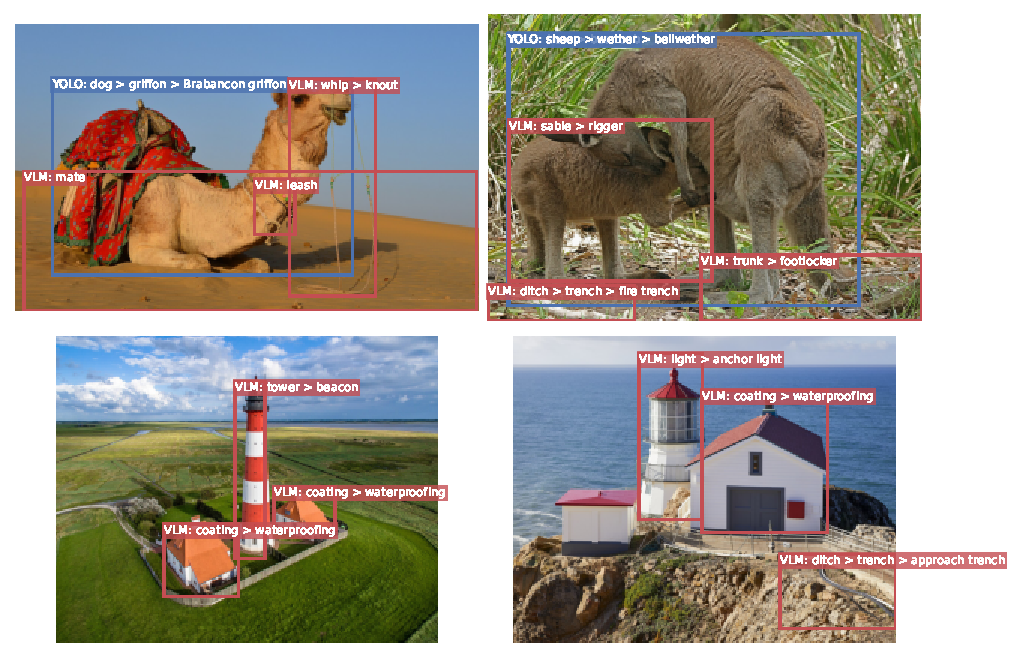
\includegraphics[width=0.85\linewidth]{figures/fig_qualitative.pdf}
    \caption{COCO外の物体を主な被写体とする実画像に対する，YOLO11xにOWLv2の候補を加えた構成の結果．青はYOLO11x（閾値0.25）のボックスとハイブリッド手法による粒度の変更，赤は加えた候補のうち物体らしさのスコアの上位3件とSigLIPによる命名と粒度の変更である．画像はWikimedia Commons（CC BY-SA 3.0/4.0）より取得した．}
    \label{fig_qualitative}
\end{figure*}
